\chapter{Strategy Pattern}

\section{Định nghĩa}
Strategy Pattern là một trong những pattern thuộc nhóm hành vi (Behavior Pattern). Strategy Pattern xác định một nhóm các thuật toán, đóng gói từng cái một và khiến cho chúng có thể hoán đổi vị trí cho nhau một cách linh hoạt bên trong object. Strategy cho phép thuật toán biến đổi độc lập khi người dùng sử dụng chúng.

\section{Mục đích sử dụng}
\begin{itemize}
\item Thay đổi các thuật toán được sử dụng bên trong một đối tượng tại thời điểm run-time.
\item Khi có một đoạn mã dễ thay đổi, và muốn tách chúng ra khỏi chương trình chính để dễ dàng bảo trì.
\item Tránh sự rắc rối khi phải hiện thực một chức năng nào đó qua quá nhiều lớp con.
\item Che giấu sự phức tạp, cấu trúc bên trong của thuật toán.
\end{itemize}

\section{Mô hình cấu trúc}
\begin{center}
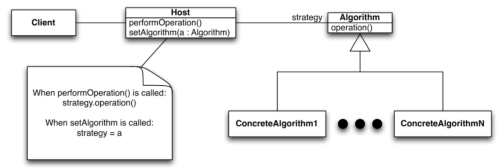
\includegraphics{GALLEYS/images/chapter9/diagram}
\end{center}
Các thành phần:
\begin{itemize}
\item Algorithm: định nghĩa các hành vi/phương thức có thể có của một Algorithm.
\item ConcreteAlgorithm : cài đặt các hành vi/phương thức cụ thể của Algorithm.
\item Host: chứa một tham chiếu đến đối tượng Algorithm và nhận các yêu cầu từ Client, các yêu cầu này sau đó được ủy quyền cho Algorithm thực hiện.
\end{itemize}

Cách tiến hành: Client (main) sử dụng Host. Algorithm được kéo ra khỏi Host. Client chỉ sử dụng giao diện công khai của Algorithm và không bị ràng buộc bởi các lớp con (concrete algorithms) cụ thể. Client có thể thay đổi hành vi của mình bằng cách chuyển đổi giữa các thuật toán cụ thể (concrete algorithms) khác nhau.

Chúng ta xét đến một ví dụ cụ thể: ứng dụng sắp xếp.
Chương trình của chúng ta cung cấp nhiều giải thuật sắp xếp khác nhau: quick sort, merge sort, selection sort, heap sort, tim sort,... Tùy theo loại dữ liệu, số lượng phần tử,... mà người dùng có thể chọn một giải thuật sắp xếp phù hợp.
\begin{center}
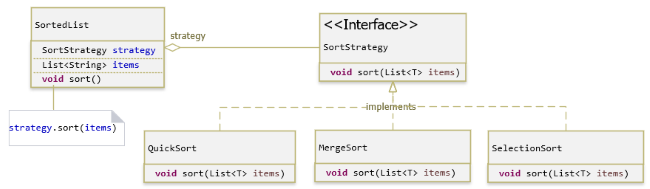
\includegraphics{GALLEYS/images/chapter9/example}
\end{center}
\newpage
\textbf{SortStrategy.java}
\begin{center}
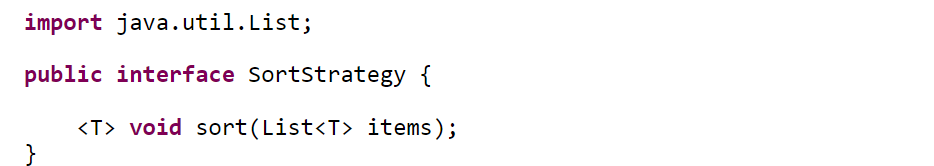
\includegraphics{GALLEYS/images/chapter9/code1}
\end{center}
\textbf{QuickSort.java}
\begin{center}
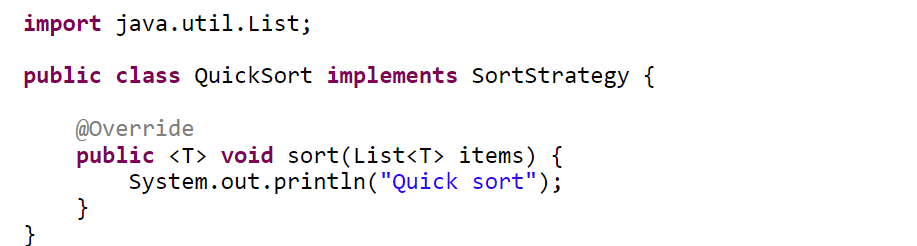
\includegraphics{GALLEYS/images/chapter9/code2}
\end{center}
\textbf{MergeSort.java}
\begin{center}
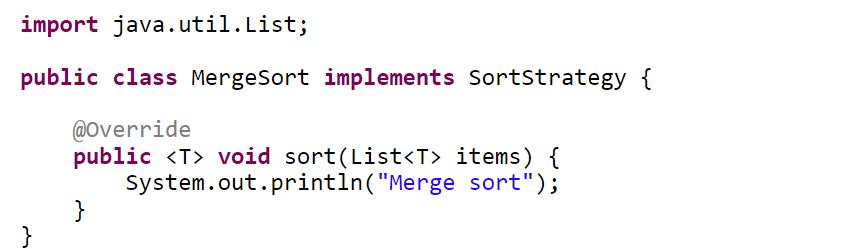
\includegraphics{GALLEYS/images/chapter9/code3}
\end{center}
\textbf{SelectionSort.java}
\begin{center}
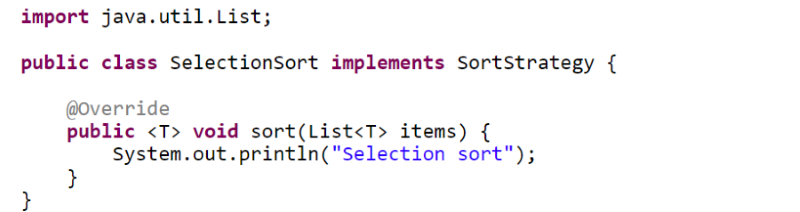
\includegraphics{GALLEYS/images/chapter9/code4}
\end{center}
\textbf{SortedList.java}
\begin{center}
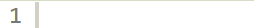
\includegraphics{GALLEYS/images/chapter9/code5}
\end{center}
\newpage
\textbf{SortStrategy.java}
\begin{center}
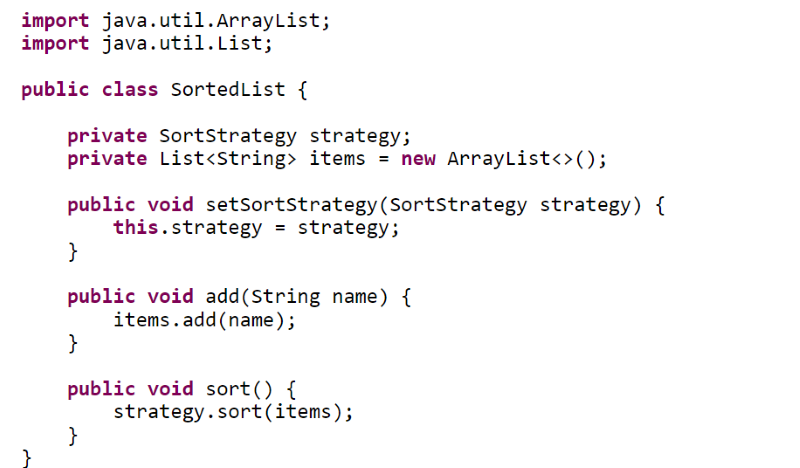
\includegraphics{GALLEYS/images/chapter9/code6}
\end{center}
\newpage
\textbf{StrategyPatternExample.java}
\begin{center}
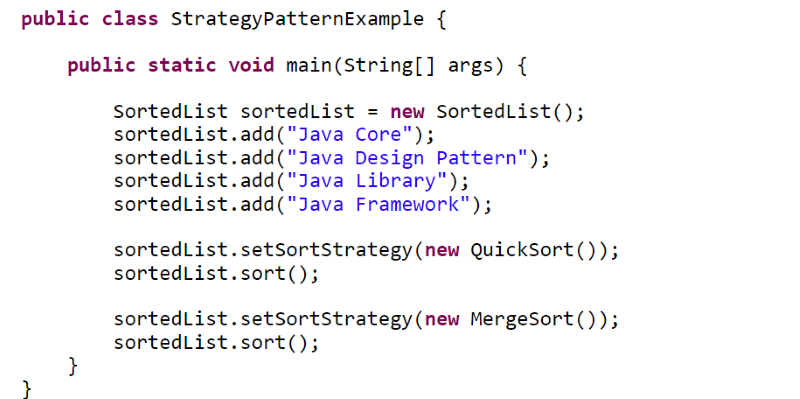
\includegraphics{GALLEYS/images/chapter9/code7}
\end{center}
\textbf{Và cuối cùng là output của chương trình:}\\
\textbf{Quick sort}\\
\textbf{Merge sort}

\section{Strategy Pattern trong thực tế}
Bất kỳ phần mềm nào cần giải quyết các tác vụ đang chờ xử lý và các vấn đề có khả năng thay đổi, các tùy chọn hành vi và các thay đổi đều là ứng cử viên chính cho Strategy Pattern.

Ví dụ: các chương trình cung cấp các định dạng lưu trữ khác nhau cho các tệp hoặc các chức năng sắp xếp và tìm kiếm khác nhau có thể sử dụng các Strategy Pattern. Tương tự như vậy trong nén dữ liệu, các chương trình được sử dụng để thực hiện các thuật toán nén khác nhau dựa trên design pattern. Bằng cách này, chúng có thể chuyển đổi các video thành định dạng tệp tiết kiệm dung lượng mong muốn hoặc khôi phục các tệp lưu trữ nén (ví dụ: tệp ZIP hoặc RAR) về trạng thái ban đầu bằng cách sử dụng các chiến lược giải nén đặc biệt (special unpacking strategies). Một ví dụ khác là lưu tài liệu hoặc hình ảnh ở các định dạng tệp khác nhau.

Hơn nữa, design pattern liên quan đến việc phát triển và triển khai phần mềm trò chơi, phần mềm này phải phản ứng linh hoạt với các tình huống trò chơi thay đổi trong thời gian chạy. Các nhân vật khác nhau, trang bị đặc biệt, hành vi của hình người hoặc các bước di chuyển khác nhau (chuyển động đặc biệt của nhân vật trò chơi) có thể được lưu trữ dưới dạng ConcreteStrategies.

Một lĩnh vực ứng dụng khác của các Strategy Pattern là phần mềm thuế. Bằng cách chuyển đổi ConcreteStrategies, mức giá có thể dễ dàng được điều chỉnh cho các nhóm chuyên nghiệp (professional groups), các quốc gia và các khu vực. Hơn nữa, các chương trình chuyển đổi dữ liệu sang các định dạng đồ họa khác nhau (ví dụ như đường, hình tròn hoặc các biểu đồ thanh) sử dụng các Strategy Pattern.

Các ứng dụng cụ thể hơn của các Strategy Pattern có thể được tìm thấy trong thư viện chuẩn Java (Java API) và trong bộ công cụ Java GUI (ví dụ: AWT, Swing và SWT), thứ mà sử dụng trình quản lý bố cục trong việc phát triển và tạo các giao diện đồ họa người dùng (GUI). Điều này có thể thực hiện các chiến lược khác nhau để cấu hình các thành phần trong phát triển giao diện. Các ứng dụng khác của các mẫu thiết kế chiến lược bao gồm các hệ thống cơ sở dữ liệu, các trình điều khiển thiết bị và các chương trình máy chủ.
